\chapter{Statistiques descriptives du jeu de données}
\section*{Division du dataset}
Le dataset a été divisé en trois parties : entraînement, validation et test. Voici la répartition du nombre de commentaires dans chacune de ces parties :
\begin{table}[h]
\centering
\begin{tabular}{lc}
\toprule
\textbf{Catégorie} & \textbf{Nombre de commentaires} \\
\midrule
Train & 127,656 \\
Validation & 31,915 \\
Test & 63,978 \\
\bottomrule
\end{tabular}
\caption{Répartition du nombre de commentaires}
\end{table}


\section*{Répartition des labels}
Les commentaires toxiques sont minoritaires dans l'ensemble des données. 
En effet il y a \textbf{10.2\%} de commentaire globalement non-toxique. 
Cela peut poser des problèmes lors de l'entraînement des modèles, car les classes minoritaires peuvent être sous-représentées et donc mal apprises.
Il y a aussi une répartition inégale au sein des labels de toxicité
On peut remarquer que la somme des pourcentages n'est pas égale à 100\% car un commentaire peut avoir plusieurs labels. 
On est donc dans un problème de classification multi-labels.
\begin{table}[h]
\centering
\begin{tabular}{lc}
\toprule
\textbf{Label} & \textbf{Pourcentage} \\
\midrule
toxic & 94.3\% \\
severe\_toxic & 9.8\% \\
obscene & 51.9\% \\
threat & 3.1\% \\
insult & 48.2\% \\
identity-hate & 8.6\% \\ % Replace X.X with the actual value
\bottomrule
\end{tabular}
\caption{Répartition des labels sur les commentaires globalement toxiques}
\end{table}


\newpage
\section*{Corrélation entre les labels}
On peut remarqué que les labels de toxicité sont fortement corrélés entre eux. 
On peut dès à présent anticiper une difficulté du modèle à distinge un commentaire toxique d'un commentaire obscene (\textbf{74\%} de corrélation).
Cela représente un point à prendre en compte lors de la conception du modèle. La matrice de corrélation est inclus dans l'appendice \ref{chap:appendix}. 

\section*{Longueur des commentaires}
La distribution de la longueur des commentaires est très variée. En effet l'écart type est bien plus élevé que la moyenne. 
La longueur moyenne des commentaires est de \textbf{395} caractères, avec un écart-type de \textbf{593} caractères. 
Cela peut poser des problèmes lors de la conception du modèle. Il est donc important de prétraiter les données pour normaliser la longueur des commentaires.
\begin{figure}[h]
    \centering
    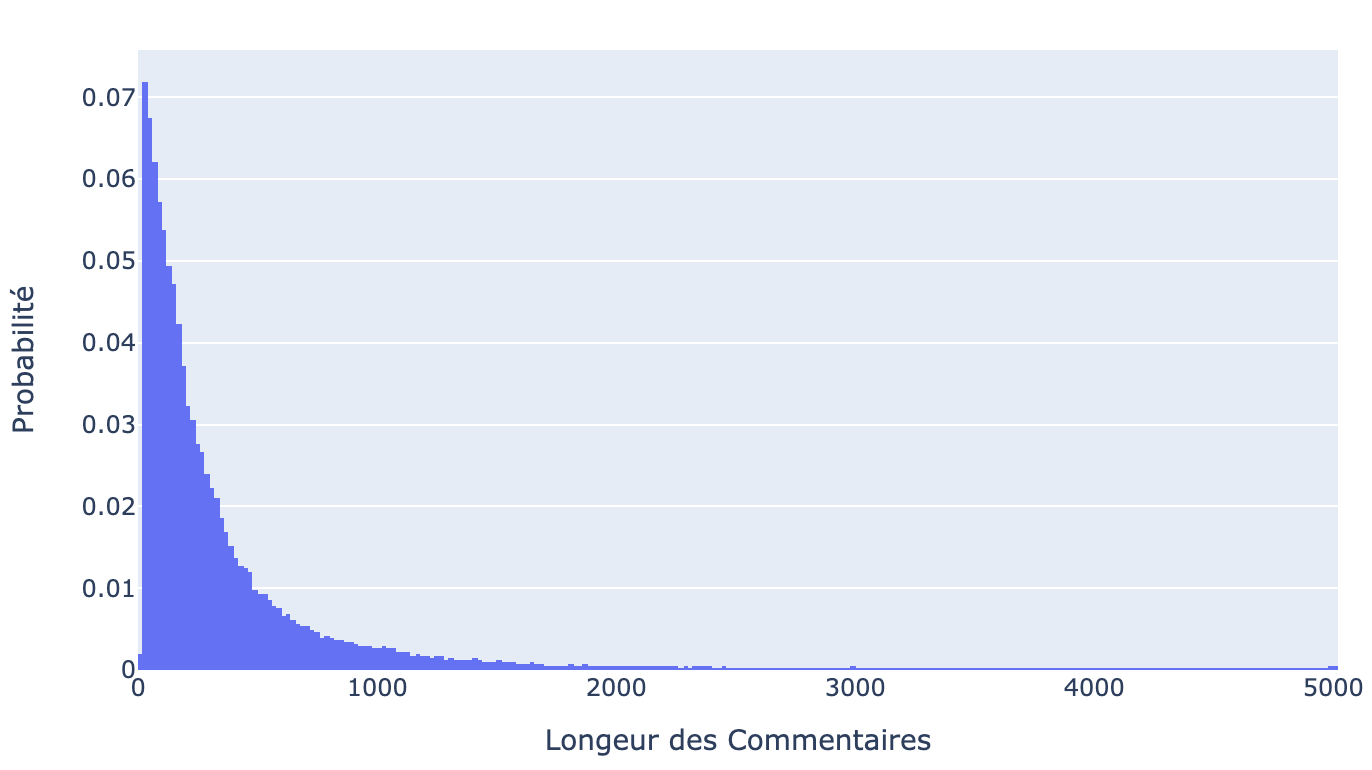
\includegraphics[width=0.5\textwidth]{figures/long-commentaire-prob.png}
    \caption{Distribution de la longueur des commentaires}
\end{figure}

\section*{Distribution des mots}
Dans le jeu de données, il y a un total de environs 180 000 mots uniques. 
Sans surprises, les mots les plus fréquents sont les mots de liaison et les mots vides. 
Mais en vue de la source du dataset les mots \textbf{articles}, \textbf{wikipedia} et \textbf{pages} apparaissent aussi très souvent dans les commentaires (top 26, 30, 31 respectivement).
En effet les utilisateurs peuvent citer des sources pour appuyer leurs propos. 
Dans les commentaires toxiques, on trouve des insultes, des mots vulgaires et des mots discriminatoires.
On peut visualiser ces derniers en utilisant WordCloud. Cela représente une représentation visuelle des mots les plus utilisés.
En annexe \ref{chap:appendix}, on peut voir une représentation WordCloud générée à partir des commentaires du jeu de données filtré selon le type de toxicité.
